% Compile with: pdflatex waveguide_rectangle_obstacle.tex
\documentclass[tikz,border=10pt]{standalone}
\usepackage{tikz}
\usepackage{amsmath}
\begin{document}

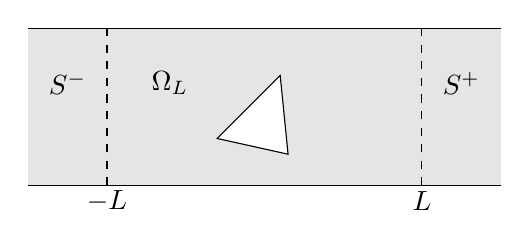
\begin{tikzpicture}[scale=1]
  % Parameters
  \def\d{2}
  \def\H{2}
  \def\L{6}

  % Waveguide rectangle (shaded)
  \fill[gray!20] (-\L/2,-\H/2) rectangle (\L/2,\H/2);

  % Dashed boundary lines for y=±H/2 (waveguide walls)
  \draw[thin] (-\L/2,-\H/2) -- (\L/2,-\H/2);
  \draw[thin] (-\L/2, \H/2) -- (\L/2, \H/2);

  % Vertical dashed lines at -d and d
  \draw[dashed] (-\d,-\H/2) -- (-\d,\H/2);
  \draw[dashed] ( \d,-\H/2) -- ( \d,\H/2);

  % Obstacle (triangle)
  \filldraw[fill=white, draw=black, thin] (-0.6,-0.4) -- (0.3,-0.6) -- (0.2,0.4) -- cycle;

  % Labels
  \node at (-1.2,0.3) {$\Omega_L$};
  \node at (-\d,-1.2) {$-L$};
  \node at ( \d,-1.2) {$L$};
  \node at (-2.5,0.3) {$S^-$};
  \node at (2.5,0.3) {$S^+$};

\end{tikzpicture}

\end{document}